% !TEX program = xelatex
\documentclass{template}
\usepackage{fontspec}
\usepackage{lipsum}
\setmainfont{Times New Roman}
\usepackage{xcolor}
\usepackage{graphicx} % Required for inserting images
\usepackage[style=ieee, backend=biber]{biblatex}
\usepackage{animate}
\addbibresource{ref.bib}
\linespread{1.5}
\renewcommand{\listfigurename}{Tableau de figures}
\usepackage{fancyhdr}
\pagestyle{fancy}
\fancyhf{}
\lhead{
\includegraphics[scale=0.2]{Pics/LogoLyon1Sig_CoulRvb72dpi.jpg}}
\rhead{ Rapport de stage – Laboratoire DISP }
\rfoot{\thepage}
\lfoot{Do Truong Thinh TRUONG – L3 Informatique}
\renewcommand{\headrulewidth}{2pt}
\renewcommand{\footrulewidth}{2pt}

\usepackage{titlesec}
\titleformat{\section}
{\color{teal}\normalfont\Large\bfseries}
{\color{teal}\thesection}{1em}{}

\begin{document}
\section*{Remercients}
Je tiens à exprimer ma gratitude envers toutes les personnes qui m'ont aidé pendant mon stage. \\ \\
Tout d'abord, je tiens à remercier le laboratoire DISP, pôle RTI pour m'avoir offert une opportunité incroyable de stage. Je suis reconnaissant pour l'expérience que j'ai acquise en travaillant avec l’équipe.\\ \\
Je tiens également à remercier M. Badreddine Tanane pour sa patience, ses conseils et son soutien tout au long de mon stage. Ses conseils, son expérience et son mentorat m'ont beaucoup aidé à développer mes compétences.\\ \\
Je voudrais aussi remercier mon tuteur académique, M. Alexandre Meyer pour son aide et sa coopération. Il m’a beaucoup aidé avec le côté administratif.\\ \\
Je suis reconnaissant envers chacun d'entre vous pour votre contribution à mon stage et pour l'impact positif qu'il a eu sur moi. Vos efforts ne seront jamais oubliés.
\newpage

%------------ Table des matières ----------------

\tabledematieres % Créer la table de matières

%------------ Table des figures ----------------

\listoffigures
\newpage 
%------------ Corps du rapport ----------------


%------------ Introduction ----------------


\section{Introduction}
\subsection{Stage en L3}
Dans le cadre de ma dernière année de Licence Informatique à l’Université Claude Bernard Lyon 1, je dois effectuer un stage d’une durée près de 3 mois. Ce stage vise à clôturer mon cursus. Il me permet d’être formé au sein d’une entreprise dans le but d’acquérir des connaissances sur un secteur d’activité, tout en me permettant de mettre en pratique les connaissances théoriques que j’ai acquises lors de mon cursus.
\subsection{Rapport de stage}
Dans ce rapport, je présente mon environnement de travail ainsi que les missions principales que j’ai au sein du laboratoire DISP, pôle RTI à IUT Lyon 2 Lumière, pour le développement d'une application IOT (Internet of Things) et IA (Intelligence Artificielle) de l'industrie 4.0. En effet, en tant que développeur full-stack, celles-là consistent de concevoir un système de l'architecture microservices et donc ses services et éventuellement le déploiement des ces services. 
\subsection{Projet du stage}
Le projet fait partie de la thèse du doctorant Bareddine Tanane, le but duquel est fournir une application aux opérateurs des machines chez l'entreprise industrielle de métallurgie une façon à contrôler tous leurs opérations, grâce aux données accueillies des sources différentes. En outre, l'application exploite l'intelligence artificielle sous la forme modèles machine learning qui s'améliorent qui aide avec le decision-making.


\newpage
\section{Environnement de travail}
\subsection{Laboratoire}
Le laboratoire DISP (Décision \& Information pour les Systèmes de Production, UR4570) réunit des chercheurs et enseignants-chercheurs de l'Université de Lyon, spécialisés en génie industriel et informatique pour l'entreprise. Leurs travaux de recherche portent sur la création et l'implémentation de méthodes pour soutenir la prise de décision et les systèmes d'information, afin d'améliorer la performance, l'agilité et la résilience des systèmes de production et des chaînes logistiques.

Le laboratoire possède une double expertise qui allie compétences en modélisation, recherche opérationnelle, simulation, génie logiciel, intelligence artificielle, planification, ordonnancement et aide à la décision. Cette approche interdisciplinaire permet d'analyser ces systèmes complexes en tenant compte des dimensions techniques, structurelles, organisationnelles et humaines.

Les membres du laboratoire DISP \cite{DISPdesc} sont répartis au sein de quatre établissements de l'Université de Lyon : l'INSA Lyon, l'Université Lumière Lyon 2, l'Université Claude Bernard Lyon 1 et l'Université Jean Monnet de Saint Étienne. Leurs activités englobent la recherche scientifique théorique et appliquée, le transfert de connaissances, la valorisation des résultats, la formation par la recherche, l'expertise et l'appui à la recherche, ainsi que la diffusion de la culture et de l'information scientifique. 
\subsection{Communication au sein de l’équipe projet}
Les membres de l’équipe projet se trouvant au même étage de l’établissement, la communication verbale est le moyen de communication privilégié. L’équipe étant très disponible, il est aisé d’obtenir des réponses rapides à des questions ponctuelles ainsi que d’obtenir des entretiens voire même des réunions. Autrement, dans le cas de non-disponibilité, il est possible de se rejoindre dans un canal Microsoft Teams pour se communiquer.
\subsection{Communication hors équipe projet}
Les stagiaires des autres doctorants dans la salle de stagiaire m'ont beaucoup aidé à m'adapter au flux de travail au laboratoire et elles m'ont apporté des connaissances du domaine Data Science, Machine Learning et IOT.
\subsection{Ressources fournies et/ou à utiliser}
Chaque stagiaire se voit attribuer un bureau dans la salle de stagiaire qui est équipé d'un ordinateur connecté au réseau du laboratoire. De plus, d'autres équipements seront fournis sur demande, par exemple, les Raspberry Pis, une VM, etc.
\newpage
\section*{Missions}

\section{Architecture du système}
\subsection{Introduction}
Dans le système, les données viennent des trois différentes sources : un système d'acquisition de données IOT qui consiste de plusieurs Raspberry Pis équipés de capteurs, les méta-données des machines industrielles et les entrées des opérateurs. Tous ces données se servent à améliorer les modèles Machine Learning qui éventuellement aideront les opérateurs à prendre des décisions. En outre, il y aurait une ou plusieurs applications pour la visualisation des données et pour saisir les entrées des opérateurs.
\begin{figure}[h!]
    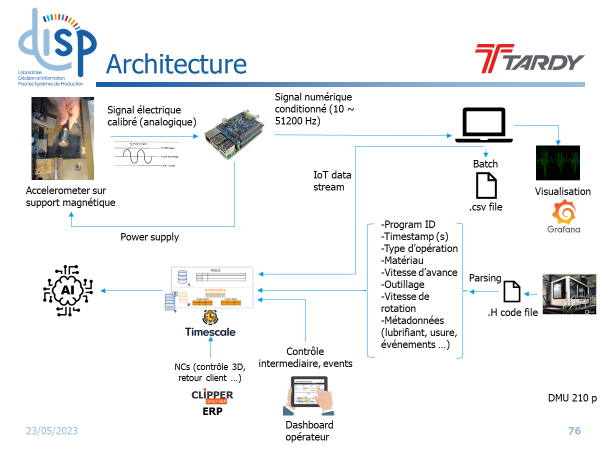
\includegraphics[scale=0.7]{Pics/SystemDataFlow.png}
    \centering
    \caption{Système de l'application}
    \label{fig:data_flow}
\end{figure}
\newpage
\subsection{Architecture Mircroservice}
Traditionnellement, le développement d'une application adopte un modèle monolithique qui consiste du développement d'une application complète en tant qu'une unité unique. Par exemple, une application traditionnelle comprendra un front-end, une API, des services, un load balancer et une base de données. Tout est construit ensemble et puis déployé sur un serveur, les services sont étroitement liés. Cela peut entraîner des difficultés lors de l'évolutivité et de la maintenance, puisque toute modification apportée à une partie du code peut affecter l'ensemble du système. En revanche, l'architecture microservices divise une application en plusieurs petits services indépendants qui interagissent les uns avec les autres. Chaque microservice est responsable d'une seule fonctionnalité, permettant ainsi une meilleure flexibilité, évolutivité et facilité de maintenance \cite{atlassianMicroservicesArchitecture} \cite{mediumArchitectureComparison}. Dans le cadre de ce projet, une architecture microservice est adoptée pour son indépendance, du développement, de langage et technologie utilisée, du scale et du déploiement de chaque service. En détail, une architecture microservice est envisagée comme ci-dessous.
\begin{figure}[h!]
    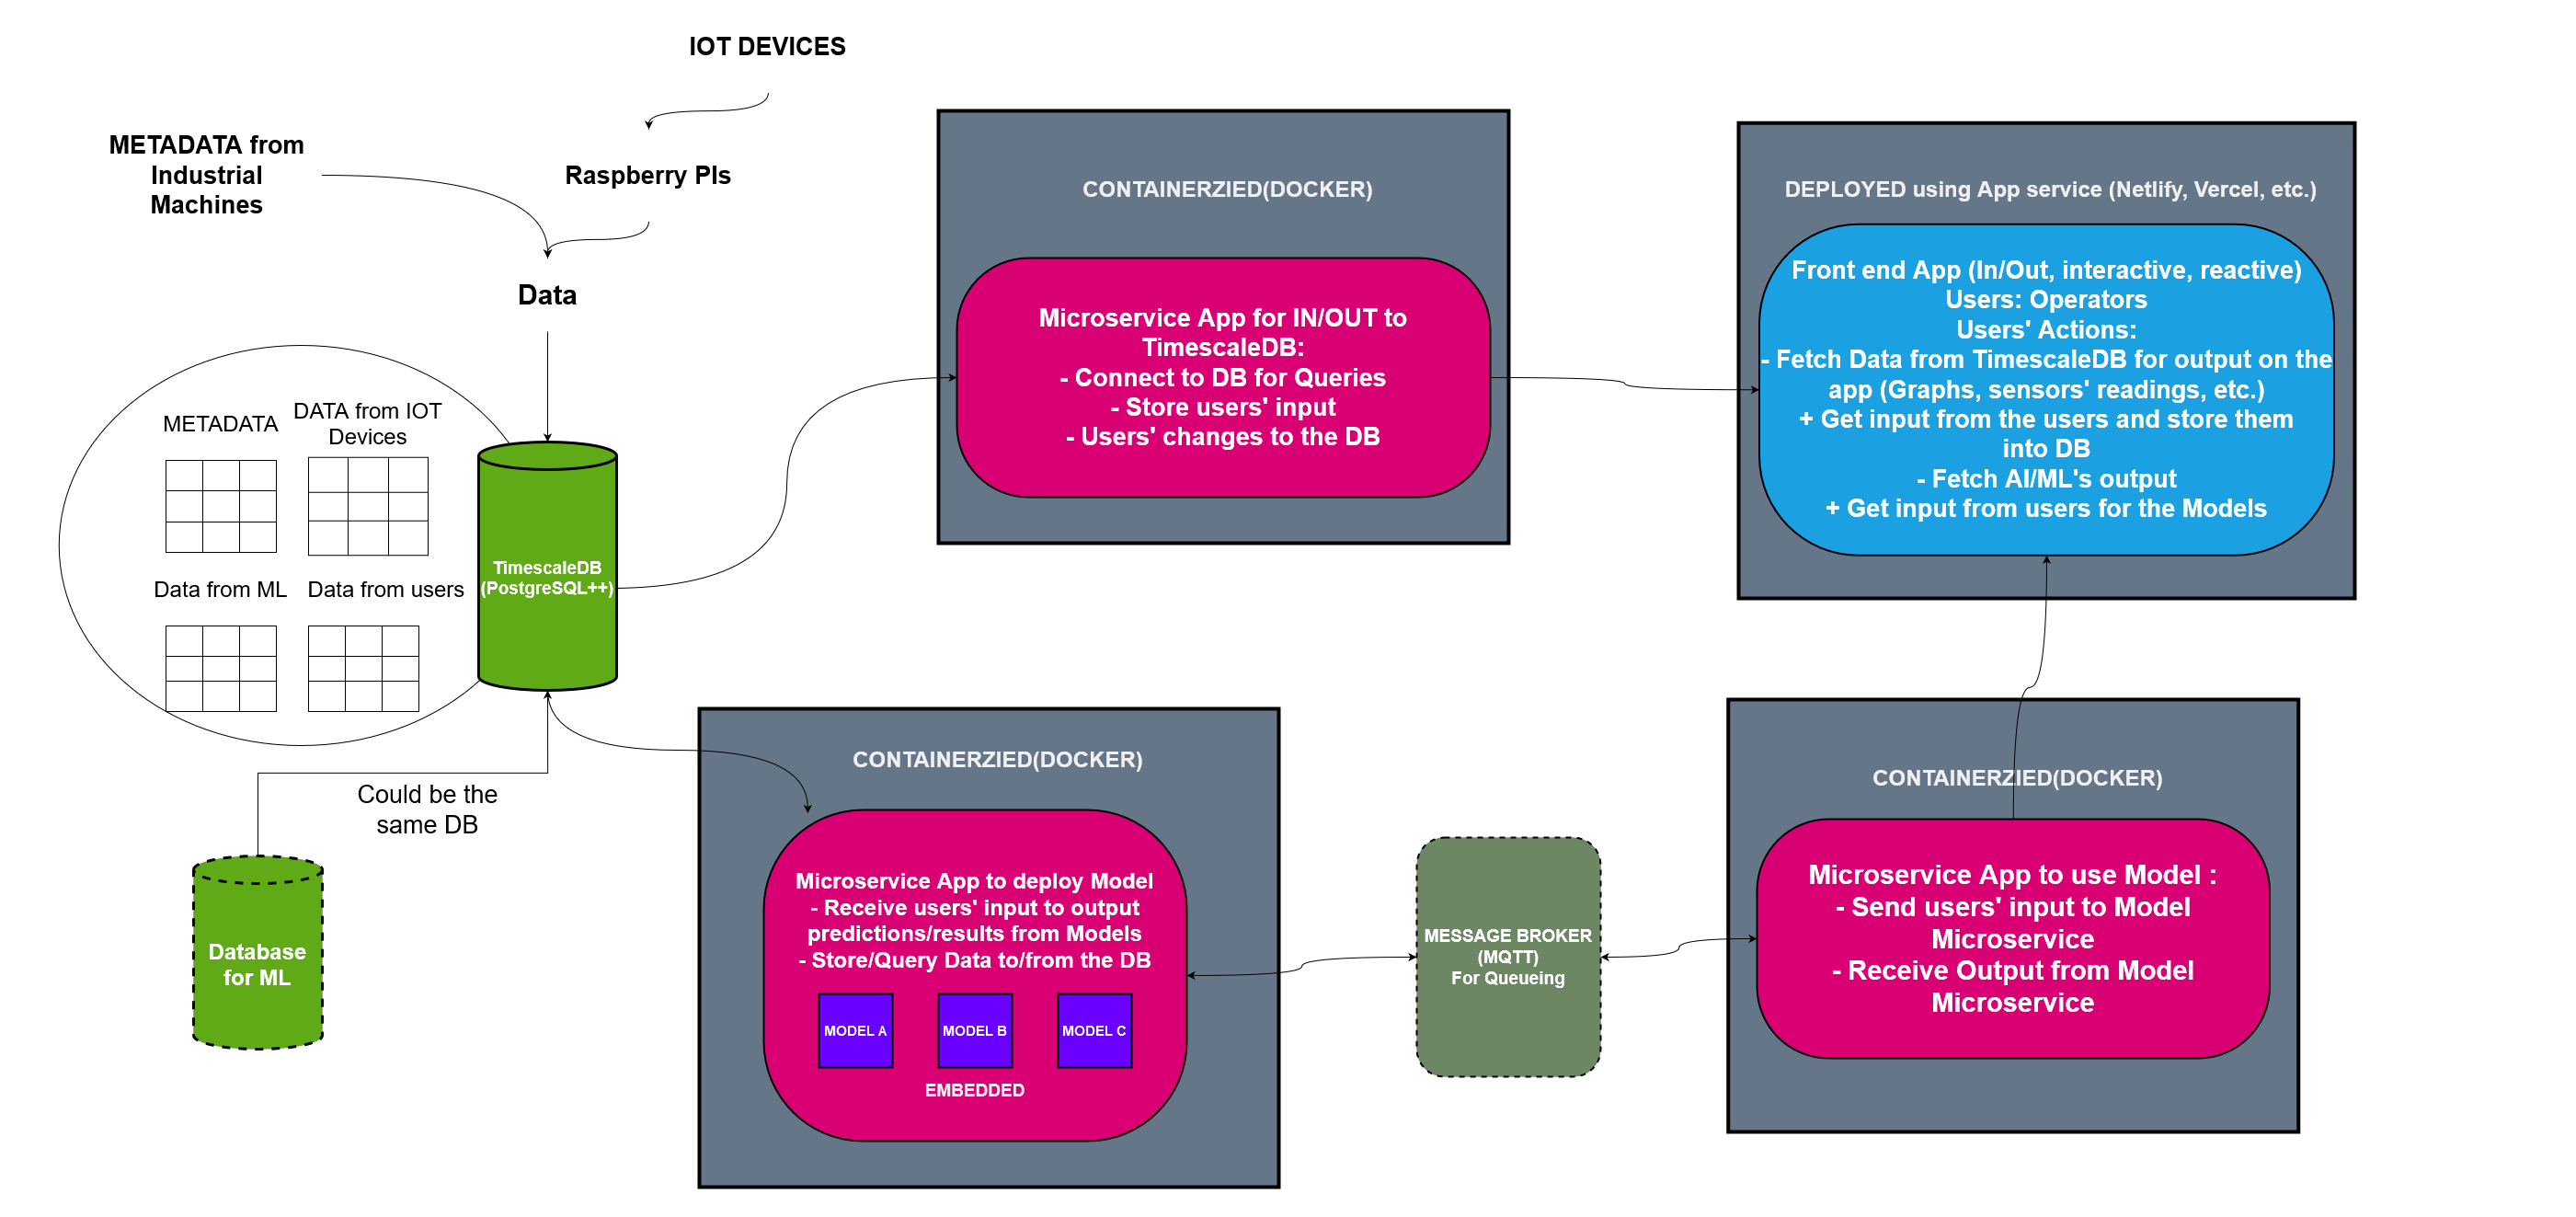
\includegraphics[scale=0.23]{Pics/SystemDesign.png}
    \centering
    \caption{Architecture Microservice de l'application}
    \label{fig:sys_des}
\end{figure}

Il y comprend essentiellement trois microservices : un pour l'entrée et la sortie des données vers les opérateurs, un pour l'utilisation des modèles ML et un pour servir et tout ce qui concerne les modèles, ensuite, une application web qui est le front-end de l'application. Chaque service fournit les APIs pour le front-end, donc chaque service est de base un serveur REST. Tous les pièces du système seront conteneurisées avec Docker pour ses déploiements.
\subsection{Conteneurisation}

De manière traditionnelle, pour faire fonctionner une application sur un ordinateur, il faut installer la version adaptée au système d'exploitation de l'appareil. Par exemple, il fallait installer la version Windows d'un logiciel sur un ordinateur sous Windows \cite{amazonQuestceConteneurisation}. Les conteneurs sont des paquets regroupant l'ensemble des éléments nécessaires au fonctionnement du logiciel, y compris le code, les dépendances, les bibliothèques, les fichiers binaires et plus encore. Docker et Kubernetes sont les frameworks les plus populaires pour orchestrer plusieurs conteneurs dans les environnements d'entreprise. Contrairement aux machines virtuelles (VM), les conteneurs partagent le noyau du système d'exploitation au lieu d'en avoir une copie intégrale, comme c'est le cas avec plusieurs VMs sur un seul hôte. Bien qu'il soit possible de déployer vos microservices sur plusieurs VMs, on utilise généralement des conteneurs dans ce cas, car ils occupent moins d'espace et démarrent plus rapidement \cite{ibmDeveloper}. Et puis, il faut avoir un outil d'orchestration qui gérera le déploiement des conteneurs qui contient les microservices.
\subsection{Orchestration}
Pour le déploiement des conteneurs, un outil orchestration est nécessaire pour éviter la complexité de les gérer à la main, cet outil rend l'automatisation d'une grande partie des efforts opérationnels requis pour exécuter des charges de travail et des services conteneurisés \cite{ibmBenefitsKubernetes}. Kubernetes (K8s) est une platforme open source très populaire qui sert à planifier et automatiser le déploiement, la gestion et la mise à l'échelle d'applications conteneurisées conteneurisées \cite{VMWare_2022}. Le diagramme ci-dessous illustre le mononode cluster K8s (c'est à dire qu'il y a qu'un serveur en termes de K8s) du système : 
\begin{figure}[h!]
    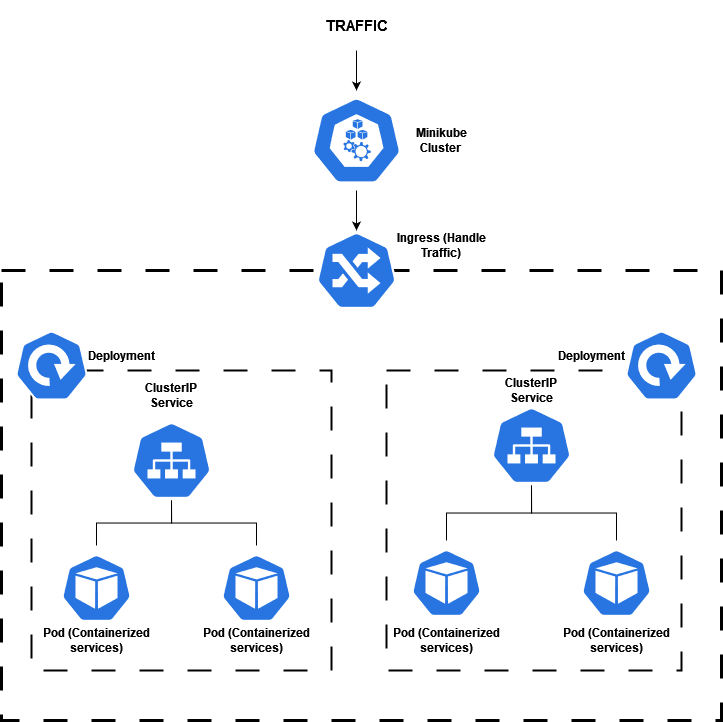
\includegraphics[scale=0.4]{Pics/K8s Diagram.png}
    \centering
    \caption{Diagramme Kubernetes Cluster}
\end{figure}
\\
Le système sera déployé sur une VM fournie par l'université Lyon 2 Lumière, où Minikube sera lancé, ce qui est une instance d'un cluster K8s qui a une node. Tous les traffiques qui viennent d'ailleurs sont réglées par Ingress, une service qui donne l'accès aux nodes du cluster et qui s'agit d'un load balancer. Dans la node, chaque service du système a son propre Deployment et Service pour son évolutivité, sa maintenance et sa connectivité, ici la Service ClusterIP aussi s'agit d'un load balancer pour les pods (instances) des conteneurs (des applications dedans).
\section{Application Dashboard}
\subsection{Introduction}
L'application est l'interface aux opérateurs des machines industrielles, qui étaient abordés ci-dessus. Ses utilisateurs peuvent voir tous les données acquises de manière user-friendly et interactive, les relevés des capteurs en temps réel. De plus, elle sert à saisir les entrées des utilisateurs pour améliorer les modèles ML qui fourniront les prédictions. Puisque l'application a besoin de l'accessiblité et de l'interactivité et en même temps l'aise du développement \cite{trioDevelopment2023}, le modèle de l'application web est adopté. 
\begin{figure}[h!]
    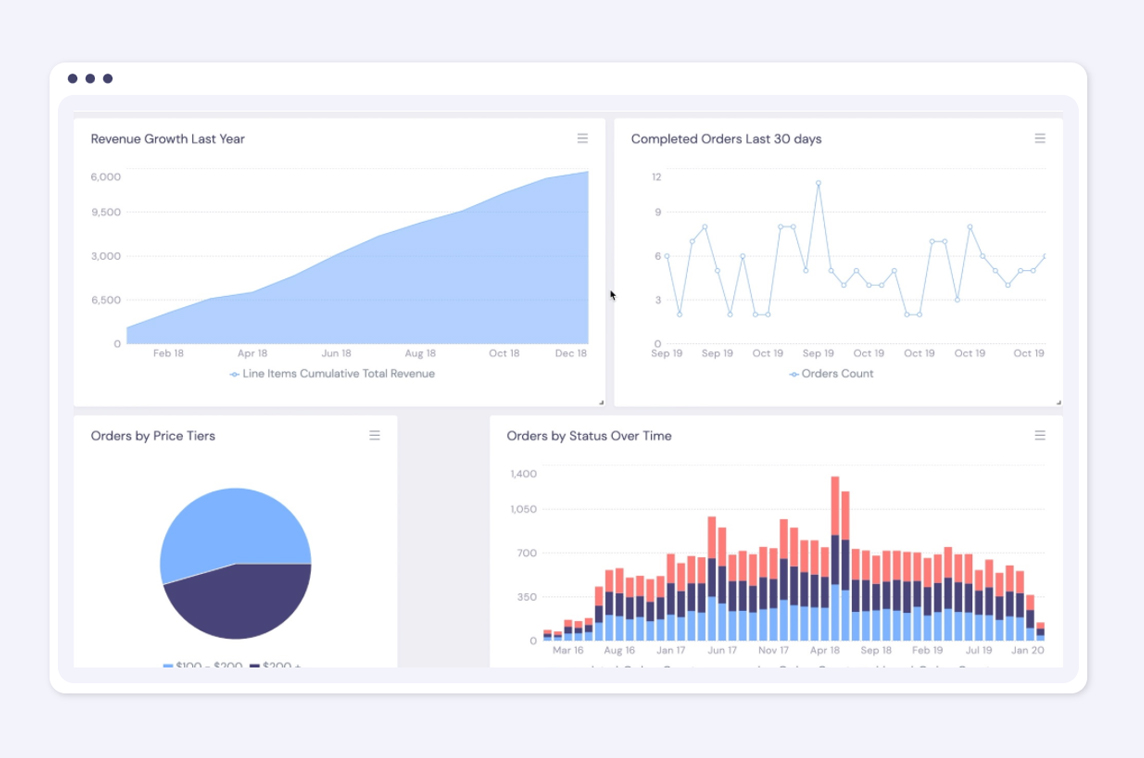
\includegraphics[scale=0.18]{Pics/react-dashboard-guide-2.jpg}
    \centering
    \caption{Exemplaire Admin Dashboard \cite{madewithreactjsReactDashboard}}
\end{figure}
\subsection{Technologies utilisées}
\subsubsection{Langage}
Certainement, JavaScript est de facto le langage pour le développement d'une application web, ce qui reste le langage le plus utilisé par la communauté des développeurs \cite{stackoverflowStackOverflow}. En outre, tous les navigateurs des appareils de nos jours supportent le JavaScript, donc il est choisi pour le développement de l'application. 
\subsubsection{ReactJS}
ReactJS est le plus populaire framework (techiniquement Meta l'appelle une librairie) front-end d'après le sondage de Stackoverflow \cite{webFrameworks} et d'après les statistiques de ce site :
\begin{figure}[h!]
    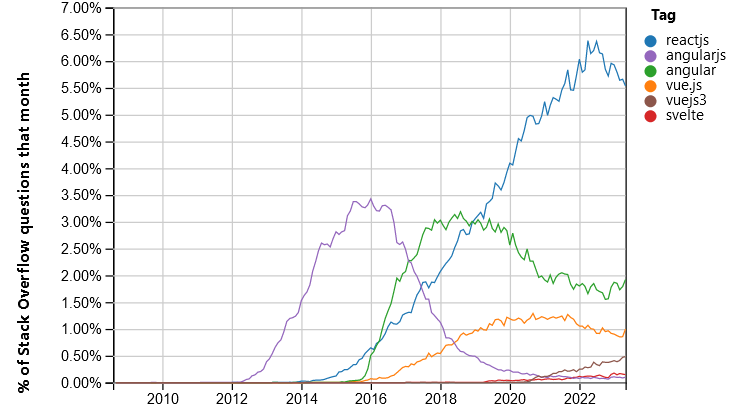
\includegraphics[scale=0.4]{Pics/stackoveflowchart.png}
    \centering
    \caption{ReactJS - Popularité \cite{stackoverflowChart}}
\end{figure}
\\
grâce à sa flexibilité, à sa performance, à sa réutilisabilité et la facilité à apprendre \cite{bocasayDveloppementQuestce}. Alors ReactJS sera utilisé en tandem avec plusieurs librairies pour développer une application interactive et performante.  
\subsubsection{Typescript}
TypeScript (TS) est un superscript de JavaScript (JS), c'est à dire que tous les codes en JavaScript sont TypeScript mais les codes en TypeScript ne sont pas JavaScript \cite{devTypeScriptBetter}. En réalité, TS prévaut sur JS grâce au fait qu'il est statiquement typé, ce qui aide avec l'expérience de développement, à implémenter la programmation orientée objet \cite{geeksforgeeksReasonsShould}, en même temps il a tous les avantages du JavaScript et la transpilation le rend compatible avec tous les librairies JS populaires et tous les navigateurs, surtout lesquels qui ne supportent que les versions anciennes de JS.
\subsubsection{Material-UI}
Material-UI est une librairie populaire de composants d'interface utilisateur (UI) pour React qui suit les principes de design de Google Material Design. Il fournit un ensemble de composants prédéfinis et personnalisables pour créer rapidement des applications web modernes et responsives. En outre, cette librarie propose une intégration facile grâce à des documents et des exemples complets et à une grande communauté de développeurs qui l'utilisent.
\begin{figure}[h!]
    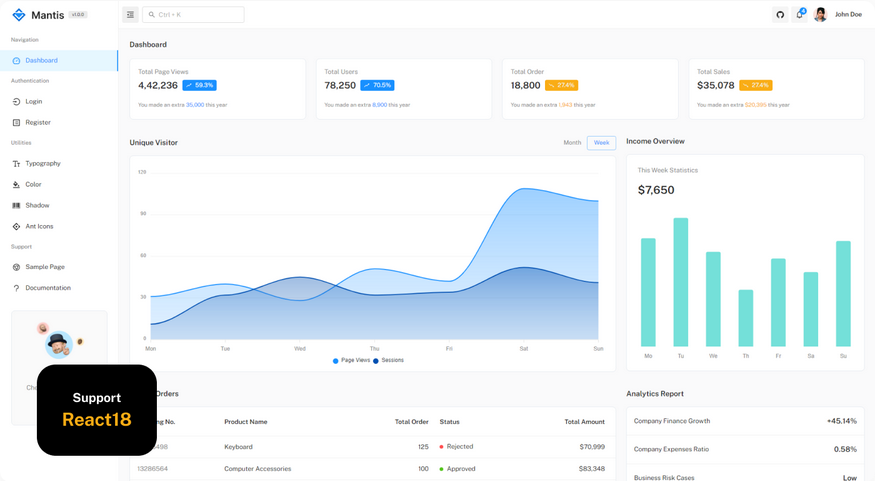
\includegraphics[scale=0.3]{Pics/mantis.png}
    \centering
    \caption{Exemplaire Material-UI Dashboard \cite{muiMantisFree}}
\end{figure}
\\
\subsubsection{Lightning Chart JS}
Lightning Chart JS (LCJS) \cite{lightningchartWorldsFastest} est une librairie pour rendre les graphes rapides, interactifs, responsifs en JavaScript grâce au support de Rendering par la carte graphique (GPU) avec la technologie WebGL. Par contre, même si LCJS est un produit commercial, il existe une version communauté qui vient avec les exemples et les guides pour intégrer les différentes types de graphe en JavaScript normal ou en plusieurs frameworks.
\section{Travail Réalisé}
\subsection{Partie Graphe}
\subsubsection{Introduction}
Le dashboard a besoin d'un streaming chart, c'est à dire un graphe qui illustre les données en live pour que les opérateurs puissent voir l'évolution de la vibration des machines industrielles en temps réel. En réalité, les graphes en temps réel ne sont pas atteignables dans le contexte d'application web vu que les applications se communique à travers Internet, le décalage est inévitable. Par contre, certaines mesures suivantes sont adoptées pour le minimiser.
\subsubsection{Réception de données}
Websockets est la technologie standard de l'industrie pour la communication en temps réel, plusieurs entreprises \cite{ablyWhatWebSockets} l'utilisent pour fournir des services qui exigent des mises à jour en temps réel, notamment Netflix pour realtime streaming, Discord pour la communication entre le client et le serveur, et plein d'autres comme Twitch, Messenger, WhatsApp, etc. Alors websockets seront utilisés pour la communication entre le client et le serveur, dans le cas de l'application, le client est l'application web (le dashboard) et le serveur est le Raspberry Pi connecté aux capteurs. 
\subsubsection{ChartJS vs. Lightning Chart JS}
D3.js \cite{d3jsObservableJavaScript} est la librairie la plus populaire en JavaScript pour créer des graphes, malheureusement, elle a besoin de manipuler le DOM directement, ce que fait aussi ReactJS, c'est pourquoi, il est difficile à intégrer les deux. Alternativement, il y a Chart.js \cite{chartjsChartjs} qui a plus de 50k étoiles sur son repo Github et qui est très réputé dans la communauté de développeurs web. En effet, cette libraire offre la création des graphes rapides, interactifs, responsifs et une variété de plugins de tiers. Dans l'implémentation suivante, les plugins chartjs-plugin-streaming \cite{nagixChartjspluginstreamingDocumentation} et chartjs-plugin-zoom \cite{chartjsChartjspluginzoom} sont utilisés pour tracer un graphe de données live : 
\begin{figure}[h!]
    \centering
    \animategraphics[autoplay, loop, width\=textwidth]{60}{chartjsgif/image-}{0}{488}
    \caption{Placeholder}
\end{figure}
Il semble que cela est parfait pour ce dont l'application a besoin, pourtant, la performance se dégradera avec le temps à tel point que l'application n'est plus réactive ou apparaît bloquée. La cause de ce problème sont normalement le fait que le graphe est re-rendu entièrement chaque fois des données nouvelles sont reçues, qui n'est pas le cas avec Chart.js, ou que tous les points de données sont rendus sur le graphe sans prendre en compte le niveau de zoom et que le rendu est effectué par le CPU, ces derniers sont ce qui se passent dans ce cas. Pour récapituler, cette partie de l'application a besoin d'une libraire qui supporte WebGL où le rendu est effectué par le GPU et qui supporte un graphe live, c'est à dire des nouvelles données sont reçues de manière très fréquente. D'où Lightning Chart JS, elle est la seule librairie qui offre une utilisation libre, qui supporte WebGL et les streaming charts hors de la boîte et qui vient avec les documents et exemples complets. Ces derniers aident les développeurs à l'intégrer facilement dans leur projet. L'implémentation ci-dessous démontre un graphe live crée avec LCJS et aussi le smart-rendering mentionné :  
\begin{figure}[h!]
    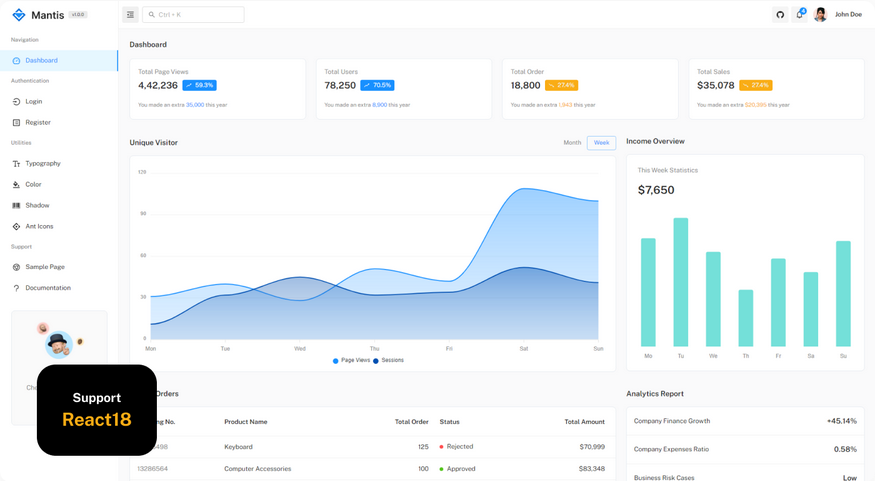
\includegraphics[scale=0.3]{Pics/mantis.png}
    \centering
    \caption{Placeholder}
\end{figure}
\newpage

\printbibliography

\newpage
\section*{Annexe}

\end{document}
